\documentclass[12pt]{article}
\usepackage{graphicx}
\usepackage{xcolor}
% \usepackage[margin=1.7cm]{geometry}
\usepackage{colortbl}
\usepackage{tikz}
\usepackage{amsmath}
\usepackage{caption}
\usepackage{subcaption}
\usepackage{textcomp}
\newcommand{\todo}[2]{{\color{red}\textbf{Todo voor #1:} #2}}
\begin{document}
\begin{titlepage}
\begin{center}
    
\includegraphics[width=\textwidth]{./logo.png}
    \\ [2.5cm]
    \textsc{\Large Autonomous Mobile Robots}
    \\ [0.5cm]
    \textsc{\large Fourth assignment}
    \\ [1cm]
    \hrule
    \vspace{0.3cm}
    \textsc{Particle Filter Based Simultaneous Localization And Mapping}
    \\ [0.3cm]
    \hrule
    \vfill
    \textsc{Ruben Janssen, 10252657 \\ David van Erkelens, 10264019 \\[0.7cm] Department of Computer Science \\ University of Amsterdam \\[0.3cm] \today \\[0.5cm] All code published on}
    \\
    \verb|www.github.com/David1209/AMR/assignment4|
\end{center}
\end{titlepage}
\tableofcontents
\clearpage
\section{Introduction}
In order for an autonomous mobile robot to be able to navigate without a priori knowlegde about the map, it has to determine its position whilst building the map. This can be accomplished by using the Simultaneous Localization and Mapping (SLAM) algorithm. One of the variations of SLAM is FastSLAM, a particle filter based algorithm which has a better performance in real time map building. FastSLAM scales logarithmically with the number of landmarks in the map, and is therefore much more suitable for real-time applications.

\section{Setup}
A NXT robot has been equipped with an omnidirectional camera. Using this NXT, a dataset of images has been made. This is a contraint of the equipment provided, since there was no NXT available to perform real-time experiments. A basic environment has been taped out, and from the point of view of the robot some snapshots have been made. 
\todo{David}{Invoegen van afbeelding van de map}  \todo{Ruben}{Iets vertellen over meegeleverde logfiles}
\section{FastSLAM}
To implement FastSLAM, a pre-recorded dataset had been provided. The input of the SLAM algorithm consists of odometry data and observable features. Here, corners are used as landmarks, detected as endpoint segments of lines extracted from data using the onmidirectional camera. The corner detection algorithm can be reduced to two steps: line extraction and endpoint collection.
\subsection{Line extraction}
A snapshot from the onmidirectional camera describes a 2D slice of the environment. Points in such a snapshot are specified in the polar coordinate system $(pi, {\theta}i)$, with the origin at the location of the camera. In order to fit a line through the points, a line is expressed in polar coordinates:
\begin{equation}
	x\cos{\alpha} + y\sin{\alpha} = r
\end{equation}
In which $-\pi < \alpha < \pi$ is the angle between the line and the x-axis, $r >= 0$ is the distance of the line to the origin and $(x, y)$ are the Cartesian coordinates of the point lying on the plane. \\ \\
In order to identify the best line segments for the obtained measurements, the Split-and-Merge algorithm is employed.
\subsection{Endpoint collection}

\subsection{Parameters}
The FastSLAM approach estimates the pose of the robots and the features using a particle filter. Each particle represents a possible robots position and its map of the environment. A few parameters of the SLAM algorithm can be tweaked, in order to improve performance of the algorihm:
\begin{enumerate}
\item \textbf{The number of particles} - saved as \verb|PARAMS.NPARTICLES|:
\item \textbf{The variance of the odometry} - saved as \verb|sigmaX| and \verb|sigmaTH|:
\item \textbf{The variance of the range sensor} - saved as \verb|sigmaR| and \verb|sigmaB|:
\end{enumerate}
\section{Experiments}
When running the algorithm on the data set provided, it returned the following result:
\begin{figure}[h!]
	\centering
	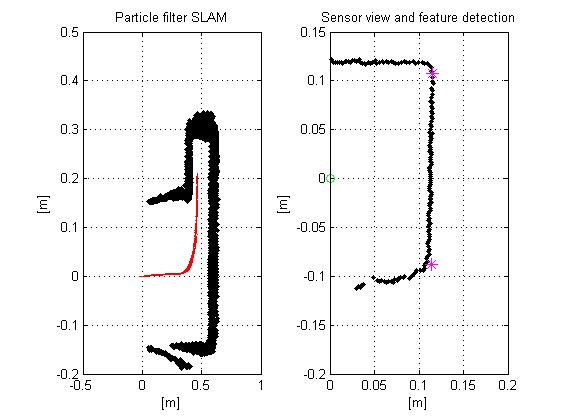
\includegraphics[width=0.5\textwidth]{normal.jpg}
\end{figure}
\section{Results}

\section{Conclusion}

\end {document}